\documentclass[a4paper,12pt]{article}

%------------------------- packages -------------------------%
\usepackage[utf8]{inputenc}
\usepackage[T5]{fontenc}
\usepackage[vietnamese]{babel}
\usepackage[unicode,hidelinks]{hyperref}    % for reference
\usepackage{graphicx}
\usepackage{tikz}
\usepackage{amsmath}
\usepackage{geometry}
\usepackage{titlesec}
\usepackage{array}
\usepackage{fancyhdr}  % Ensure this is loaded last
\usepackage{lastpage}
\usepackage{setspace}
\usepackage{longtable}
\usetikzlibrary{calc}
\usepackage{tabularx}
\usepackage{array}  % For customizing row height
\usepackage{multirow} %dùng cho phần vẽ bảng ở phần lý thuyết
\usepackage[utf8]{inputenc}
\usepackage[utf8]{vietnam}
\usepackage{enumitem}
\usepackage{adjustbox}
\usepackage{amsmath,amsfonts,amssymb}
\usepackage{float}
\usepackage{array}
\usepackage{listings}
\usepackage{tcolorbox}
\usepackage{caption}
\usepackage{inconsolata}
\usepackage{listings}
\usepackage{tocloft} % for customizing TOC
\usepackage{indentfirst} % Bắt buộc đoạn đầu tiên sau tiêu đề phải thụt đầu dòng
\usepackage{subcaption}
\setlength{\parindent}{1.5em} % Thiết lập độ rộng thụt vào (có thể chỉnh thành 1cm, 2em...)

% for code and result
\lstset{
  breaklines=true,
  breakatwhitespace=true,
  basicstyle=\ttfamily\small, % Dùng font chữ nhỏ hơn
  columns=fullflexible
}
\usepackage[svgnames]{xcolor} % Cung cấp nhiều màu sắc hơn
\tcbset{
  colback=AliceBlue,       % Màu nền xanh rất nhạt
  colframe=SteelBlue,      % Màu viền xanh dương đậm
  coltitle=MidnightBlue,   % Màu tiêu đề xanh đen
  coltext=DarkSlateGray,   % Màu chữ chính
  fonttitle=\bfseries      % Font chữ in đậm cho tiêu đề
}


%------------------------- set up -------------------------%
% Set the margins
\geometry{
    left=2cm,
    right=2cm,
    top=2.5cm,
    bottom=2.5cm,
}

%------------------------- header & footer -------------------------%
\renewcommand{\headrulewidth}{0.5pt}
\renewcommand{\footrulewidth}{0.5pt}
\setlength{\headheight}{30pt}
\pagestyle{fancy}

\fancyhead{}    % clear all header fields
\fancyhead[L]{
    \begin{tabular}{ll}
        \begin{picture}(10,10)
            \put(0,-7){
\includegraphics[width=8mm]{pictures/hcmut.png}}
        \end{picture}&
        \begin{tabular}{l}
            {\ttfamily Trường Đại học Bách Khoa Tp. Hồ Chí Minh} \\
            {\ttfamily Khoa Khoa học và Kỹ thuật Máy tính} \\
        \end{tabular} 	
    \end{tabular}
}

\fancyfoot{}    % clear all footer fields

\fancyfoot[R]{\footnotesize {\ttfamily Trang {\thepage}/\pageref{LastPage}}}

%------------------------- title format settings -------------------------%
\titleformat{\chapter}[display]
  {\normalfont\huge\bfseries}{\chaptertitlename\ \thechapter}{20pt}{\Huge}

% Multi-layered Blue Border Definition
\newcommand{\coverpageborder}{
    \begin{tikzpicture}[remember picture,overlay,inner sep=0,outer sep=0]
        \draw[blue!70!black,line width=4pt] 
            ([xshift=-1.5cm,yshift=-2cm]current page.north east) coordinate (A)--([xshift=1.5cm,yshift=-2cm]current page.north west) coordinate(B)--([xshift=1.5cm,yshift=2cm]current page.south west) coordinate (C)--([xshift=-1.5cm,yshift=2cm]current page.south east) coordinate(D)--cycle;
        \draw ([yshift=0.5cm,xshift=-0.5cm]A)-- ([yshift=0.5cm,xshift=0.5cm]B)--
        ([yshift=-0.5cm,xshift=0.5cm]B) --([yshift=-0.5cm,xshift=-0.5cm]B)--([yshift=0.5cm,xshift=-0.5cm]C)--([yshift=0.5cm,xshift=0.5cm]C)--([yshift=-0.5cm,xshift=0.5cm]C)-- ([yshift=-0.5cm,xshift=-0.5cm]D)--([yshift=0.5cm,xshift=-0.5cm]D)--([yshift=0.5cm,xshift=0.5cm]D)--([yshift=-0.5cm,xshift=0.5cm]A)--([yshift=-0.5cm,xshift=-0.5cm]A)--([yshift=0.5cm,xshift=-0.5cm]A);
        \draw ([yshift=-0.3cm,xshift=0.3cm]A)-- ([yshift=-0.3cm,xshift=-0.3cm]B)--
        ([yshift=0.3cm,xshift=-0.3cm]B) --([yshift=0.3cm,xshift=0.3cm]B)--([yshift=-0.3cm,xshift=0.3cm]C)--([yshift=-0.3cm,xshift=-0.3cm]C)--([yshift=0.3cm,xshift=-0.3cm]C)-- ([yshift=0.3cm,xshift=0.3cm]D)--([yshift=-0.3cm,xshift=0.3cm]D)--([yshift=-0.3cm,xshift=-0.3cm]D)--([yshift=0.3cm,xshift=-0.3cm]A)--([yshift=0.3cm,xshift=0.3cm]A)--([yshift=-0.3cm,xshift=0.3cm]A);
    \end{tikzpicture}
}

%------------------------- tocloft settings -------------------------%
\renewcommand{\listfigurename}{DANH MỤC HÌNH ẢNH}


\setlength{\cftbeforesecskip}{0pt} % Space before each section entry
\setlength{\cftsecnumwidth}{2em}   % Width of the section number
\setlength{\cftsubsecindent}{3em}  % Indentation for subsections
\setlength{\cftsubsecnumwidth}{3em}% Width of the subsection number
\setlength{\cftsubsubsecindent}{5em} % Indentation for subsubsections
\setlength{\cftsubsubsecnumwidth}{4em} % Width of the subsubsection number

%------------------------- body -------------------------%
\begin{document}

%-------------------- cover --------------------%
\begin{titlepage}
    \centering
    
    % Draw the cover page border
    \coverpageborder
    
    % University and Department Info
    \textbf{\large{ĐẠI HỌC QUỐC GIA THÀNH PHỐ HỒ CHÍ MINH}}\\[0.1cm]
    \textbf{\large{TRƯỜNG ĐẠI HỌC BÁCH KHOA}}\\[0.1cm]
    \textbf{\large{KHOA KHOA HỌC VÀ KỸ THUẬT MÁY TÍNH}}\\[0.25cm]
    
    % Logo Positioning
    
\includegraphics[width=0.5\textwidth]{pictures/hcmut.png}\\[0.3cm]
    
    % Title and Subtitle
    \textbf{\LARGE{BÁO CÁO BTL}}\\[0.2cm]
    \textbf{\Large{Phát triển Ứng dụng Internet of Things}}\\[0.1cm]
    \textbf{\Large{CO3037}}\\[0.6cm]
    
    % Group Info
    \textbf{\large{Lớp: A01}}\\[0.2cm]
    \textbf{\large{GVHD: Lê Trọng Nhân}}\\[0.2cm]
    \begin{table}[h]
    \renewcommand{\arraystretch}{1.5}  % Điều chỉnh chiều cao hàng (1.5 lần bình thường)
    \centering
    \begin{adjustbox}{max width=\textwidth} % Đảm bảo bảng vừa với chiều rộng trang
    \begin{tabular}{|c|l|c|c|c|}
            \hline
            \textbf{STT} & \multicolumn{1}{c|}{\textbf{Họ và tên}} & \textbf{MSSV} & \textbf{Tên lớp} & \textbf{Tên ngành} \\ \hline
            1 & Nguyễn Thanh Toàn & 2313492 & TN01 & Kỹ thuật máy tính \\ \hline
            2 & Lê Công Vinh & 2313912 & TN01 & Kỹ thuật máy tính \\ \hline
        \end{tabular}
        \end{adjustbox}
    \end{table}
        
    \vspace{2cm} % Adjust space between the table and the advisor section
   
    
    % Date
    \textbf{\large{THÀNH PHỐ HỒ CHÍ MINH, THÁNG 4 NĂM 2026}}
\end{titlepage}


%------------------------- re-apply fancy page style -------------------------%
\pagestyle{fancy}

%------------------------- sections -------------------------%


\newpage
\setstretch{1.25}
\renewcommand{\baselinestretch}{1.25}

%=================== BODY CONTENT ===================%

% \newpage
\setstretch{1.25}
\tocloftpagestyle{fancy}
\tableofcontents


\newpage


\cleardoublepage
\addcontentsline{toc}{section}{\listfigurename} % Đưa danh mục hình ảnh vào mục lục
\listoffigures
\newpage


% --- MAIN SECTION ---
\section{Giới thiệu chung}
\subsection{Mục tiêu dự án}
\subsection{Phạm vi thực hiện}
\subsection{Phân công nhiệm vụ thành viên}


\section{Thiết kế hệ thống}
\subsection{Kiến trúc hệ thống}
\subsection{Sơ đồ khối và luồng dữ liệu}
\subsection{Danh sách linh kiện phần cứng}


\section{Triển khai các Task}
\subsection{Task 1,2, 3: Thu thập dữ liệu và trực quan hóa}
\subsubsection{Tiến trình Thu thập Dữ liệu}
Nội dung trọng tâm được triển khai trong phần này là xây dựng cơ chế thu thập thông tin khí hậu chính xác từ cảm biến kỹ thuật số DHT20. Sau quá trình thu thập dữ liệu, tất cả những thông tin về nhiệt độ và độ ẩm sẽ được lưu trữ trong Message Queue. Từ đấy toàn bộ dữ liệu sẽ được hệ thống phân tích và biểu diễn đa dạng thông qua các giao diện phần cứng khác nhau: từ việc hiển thị ký tự trên màn hình LCD cho đến việc sử dụng các trạng thái ánh sáng của LED đơn và LED RGB, qua đó tạo ra một hệ thống trực quan hóa dữ liệu sinh động và dễ dàng quan sát.

\subsubsection{Hiển thị trên LED đơn với các trạng thái nhiệt độ khác nhau}
Tác vụ quản lý thiết bị hiển thị LED đơn chịu trách nhiệm biểu diễn trạng thái nhiệt độ thông qua các nhịp điệu chớp tắt khác nhau. Hệ thống phân loại điều kiện môi trường dựa trên kiểu liệt kê \texttt{LEDBlinkyState\_t} với năm cấp độ riêng biệt. Mỗi cấp độ sẽ tương ứng với một khoảng thời gian được bộ định thời của hệ điều hành quản lý chặt chẽ nhằm đảm bảo tính chính xác về mặt thời gian thực.


\begin{figure}[H]
    \centering
    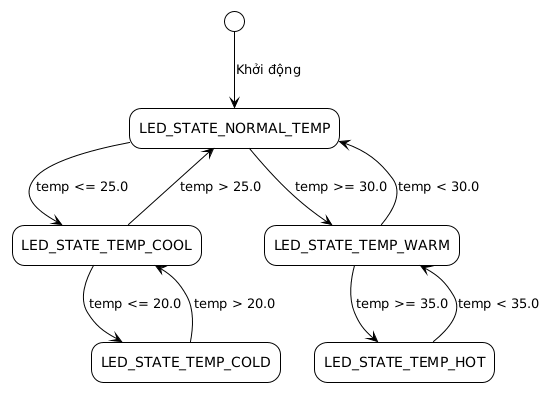
\includegraphics[width=1\textwidth]{pictures/FSM_LED.png}
    \caption{FSM các trạng thái của LED đơn tương ứng với từng mức nhiệt độ}
\end{figure}


\begin{itemize}
    \item \textbf{\texttt{LED\_STATE\_TEMP\_HOT}:} Trạng thái này xuất hiện khi nhiệt độ đo được vượt ngưỡng 35$^\circ$C. Để cảnh báo tình trạng quá nhiệt nghiêm trọng, đèn LED sẽ được điều khiển chớp tắt với tần suất cực nhanh là 100 mili giây cho mỗi chu kỳ.
    \item \textbf{\texttt{LED\_STATE\_TEMP\_WARM}:} Khi nhiệt độ nằm trong khoảng từ 30$^\circ$C đến dưới 35$^\circ$C, hệ thống xác định đây là vùng cảnh báo mức độ thấp. Nhịp điệu của đèn LED lúc này được duy trì ổn định ở mức 300 mili giây.
    \item \textbf{\texttt{LED\_STATE\_NORMAL\_TEMP}:} Đây là dải nhiệt độ lý tưởng cho vận hành, được xác lập khi giá trị đo được nằm giữa 25$^\circ$C và 30$^\circ$C. Đèn LED duy trì nhịp chớp tắt tiêu chuẩn là 1000 mili giây để biểu thị hệ thống đang hoạt động trong điều kiện bình thường.
    \item \textbf{\texttt{LED\_STATE\_TEMP\_COOL}:} Trong trường hợp môi trường trở nên mát mẻ hơn với nhiệt độ từ trên 20$^\circ$C đến 25$^\circ$C, hệ thống sẽ chuyển sang trạng thái này. Tần suất hoạt động của đèn sẽ chậm lại đáng kể với chu kỳ là 2000 mili giây.
    \item \textbf{\texttt{LED\_STATE\_TEMP\_COLD}:} Đây là mức nhiệt độ thấp nhất khi giá trị xuống dưới hoặc bằng 20$^\circ$C. Hệ thống phát tín hiệu bằng cách chớp tắt LED rất chậm với khoảng thời gian lên đến 3000 mili giây giữa các lần chuyển đổi trạng thái.
\end{itemize}

Ngoài ra, việc điều khiển chân tín hiệu của LED còn chịu ảnh hưởng trực tiếp từ tín hiệu RPC được gửi từ app.coreiot.io. Các tín hiệu đó sẽ làm thay đổi \texttt{xSemaphoreLedControl}. Chỉ khi lấy được thành công Semaphore này, hệ thống cho phép LED hoạt động dựa trên logic thời gian như trên và sau đó hoàn trả quyền điều khiển. Ngược lại nếu không lấy được Semaphore, đèn LED đơn sẽ bị ép về trạng thái tắt.

\subsubsection{Hiển thị RGB LED tương ứng với các trạng thái độ ẩm khác nhau}
Phân hệ hiển thị đa sắc sử dụng dải RGB LED để cung cấp cái nhìn trực quan về độ ẩm không khí hiện tại và trạng thái mạng. Các trạng thái màu sắc được định nghĩa thông qua kiểu dữ liệu \texttt{NeoBlinkyState\_t} và phụ thuộc chặt chẽ vào độ ẩm hiện tại. Trong khi đó, trạng thái bật tắt của đèn sẽ do trạng thái kết nối mạng hiện tại quyết định.


\begin{figure}[H]
    \centering
    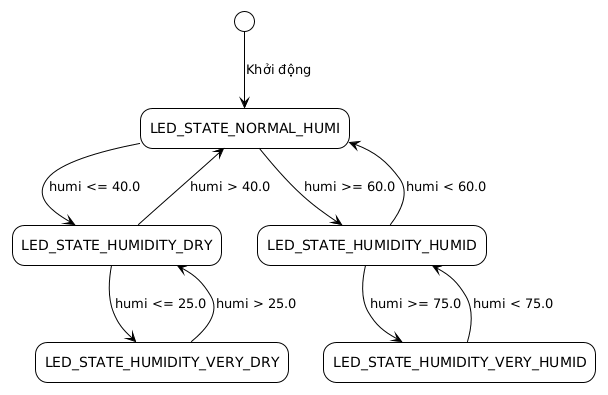
\includegraphics[width=1\textwidth]{pictures/FSM_NEO.png}
    \caption{FSM các trạng thái của RGB LED tương ứng với từng mức độ ẩm}
\end{figure}


\begin{itemize}    
    \item \textbf{Quản lý trạng thái kết nối:} Hệ thống ưu tiên kiểm tra cờ trạng thái của Semaphore kết nối mạng \texttt{xBinarySemaphoreInternet}. Nếu mất tín hiệu đường truyền, thiết bị sẽ phản hồi bằng cách cho dải LED chớp tắt liên tục mỗi 500 mili giây. Điểm đặc biệt là trong pha sáng, màu sắc vẫn phản ánh đúng mức độ ẩm hiện tại để người dùng không bị gián đoạn việc giám sát môi trường. Khi kết nối ổn định, dải LED sẽ chuyển sang chế độ sáng liên tục với màu sắc tương ứng.
    
    \item \textbf{Phân loại theo mức độ ẩm:} Màu sắc của dải LED được nội suy theo năm vùng giá trị cụ thể như sau:
    \begin{itemize}     
        \item \textbf{\texttt{LED\_STATE\_HUMIDITY\_VERY\_HUMID}:} Khi độ ẩm đạt mức rất cao từ 75\% trở lên, đèn chuyển sang màu Tím nhằm cảnh báo độ ẩm không khí các ở mức cao.
        \item \textbf{\texttt{LED\_STATE\_HUMIDITY\_HUMID}:} Với dải độ ẩm từ 60\% đến dưới 75\%, hệ thống hiển thị màu Lam để biểu thị môi trường đang ở mức khá ẩm ướt.
        \item \textbf{\texttt{LED\_STATE\_NORMAL\_HUMI}:} Màu Lục được chọn để biểu thị dải độ ẩm bình thường, dao động từ 40\% đến dưới 60\%.
        \item \textbf{\texttt{LED\_STATE\_HUMIDITY\_DRY}:} Khi không khí bắt đầu khô hanh với độ ẩm từ 25\% đến dưới 40\%, đèn sẽ chuyển sang màu Vàng để nhắc nhở người dùng.
        \item \textbf{\texttt{LED\_STATE\_HUMIDITY\_VERY\_DRY}:} Nếu độ ẩm rơi xuống mức cực thấp dưới 25\%, hệ thống lập tức hiển thị màu Đỏ để cảnh báo về điều kiện môi trường quá khô.
    \end{itemize}
\end{itemize}

\subsubsection{Hiển thị LCD}
Màn hình tinh thể lỏng đóng vai trò là trung tâm thông báo chi tiết của hệ thống. Dựa trên các thông số thu thập được, máy trạng thái của màn hình được điều khiển thông qua cấu trúc liệt kê \texttt{LCDState\_t} với ba chế độ hoạt động có tính phân cấp:

\begin{figure}[H]
    \centering
    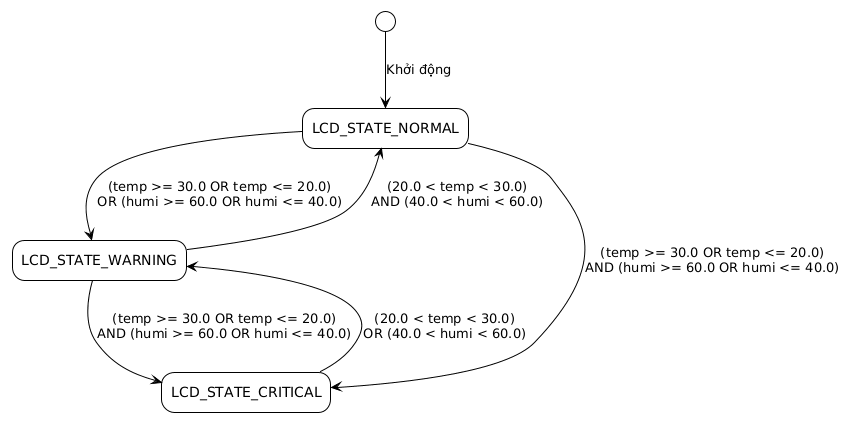
\includegraphics[width=1\textwidth]{pictures/FSM_LCD.png}
    \caption{FSM các trạng thái của LCD}
\end{figure}

\begin{itemize}
    \item \textbf{\texttt{LCD\_STATE\_NORMAL}:} Trong điều kiện môi trường ổn định, màn hình hiển thị trực tiếp các con số về nhiệt độ và độ ẩm một cách rõ ràng. Nội dung được định dạng lại để tối ưu hóa không gian hiển thị vốn hạn hẹp của các dòng ký tự, giúp người dùng nắm bắt nhanh các thông số cơ bản.
    \item \textbf{\texttt{LCD\_STATE\_WARNING}:} Khi một trong hai chỉ số môi trường bắt đầu rời khỏi vùng lý tưởng, hệ thống sẽ tự động chèn thêm thông điệp cảnh báo SOS ngay phía sau giá trị đo được. Việc này tạo ra một sự thay đổi trực quan trên giao diện hiển thị nhằm thu hút sự chú ý của người quan sát mà không làm mất đi các thông tin đo lường cần thiết.
    \item \textbf{\texttt{LCD\_STATE\_CRITICAL}:} Đây là trạng thái báo động cao nhất khi nhiệt độ hoặc độ ẩm chạm tới các ngưỡng cực đoan. Lúc này, màn hình sẽ chuyển sang chế độ nhấp nháy liên tục toàn bộ nội dung hoặc đèn nền. Sự thay đổi trạng thái thị giác mạnh mẽ này là phương thức cảnh báo cấp bách nhất, yêu cầu người vận hành phải có biện pháp can thiệp ngay lập tức để bảo vệ thiết bị hoặc điều chỉnh môi trường.
\end{itemize}




\subsection{Task 4: Web Server in Access Point Mode}

\subsection{Task 5: TinyML Deployment \& Accuracy Evaluation}

\subsection{Task 6: Data Publishing to CoreIOT Cloud Server}
\subsubsection{Dashboard}

Dashboard được thiết kế trên nền tảng Collect nhằm mục đích trực quan hóa dữ liệu thời gian thực từ các thiết bị ESP32, giúp người dùng dễ dàng theo dõi trạng thái môi trường và đưa ra các quyết định điều khiển kịp thời.

\begin{figure}[H]
    \centering
    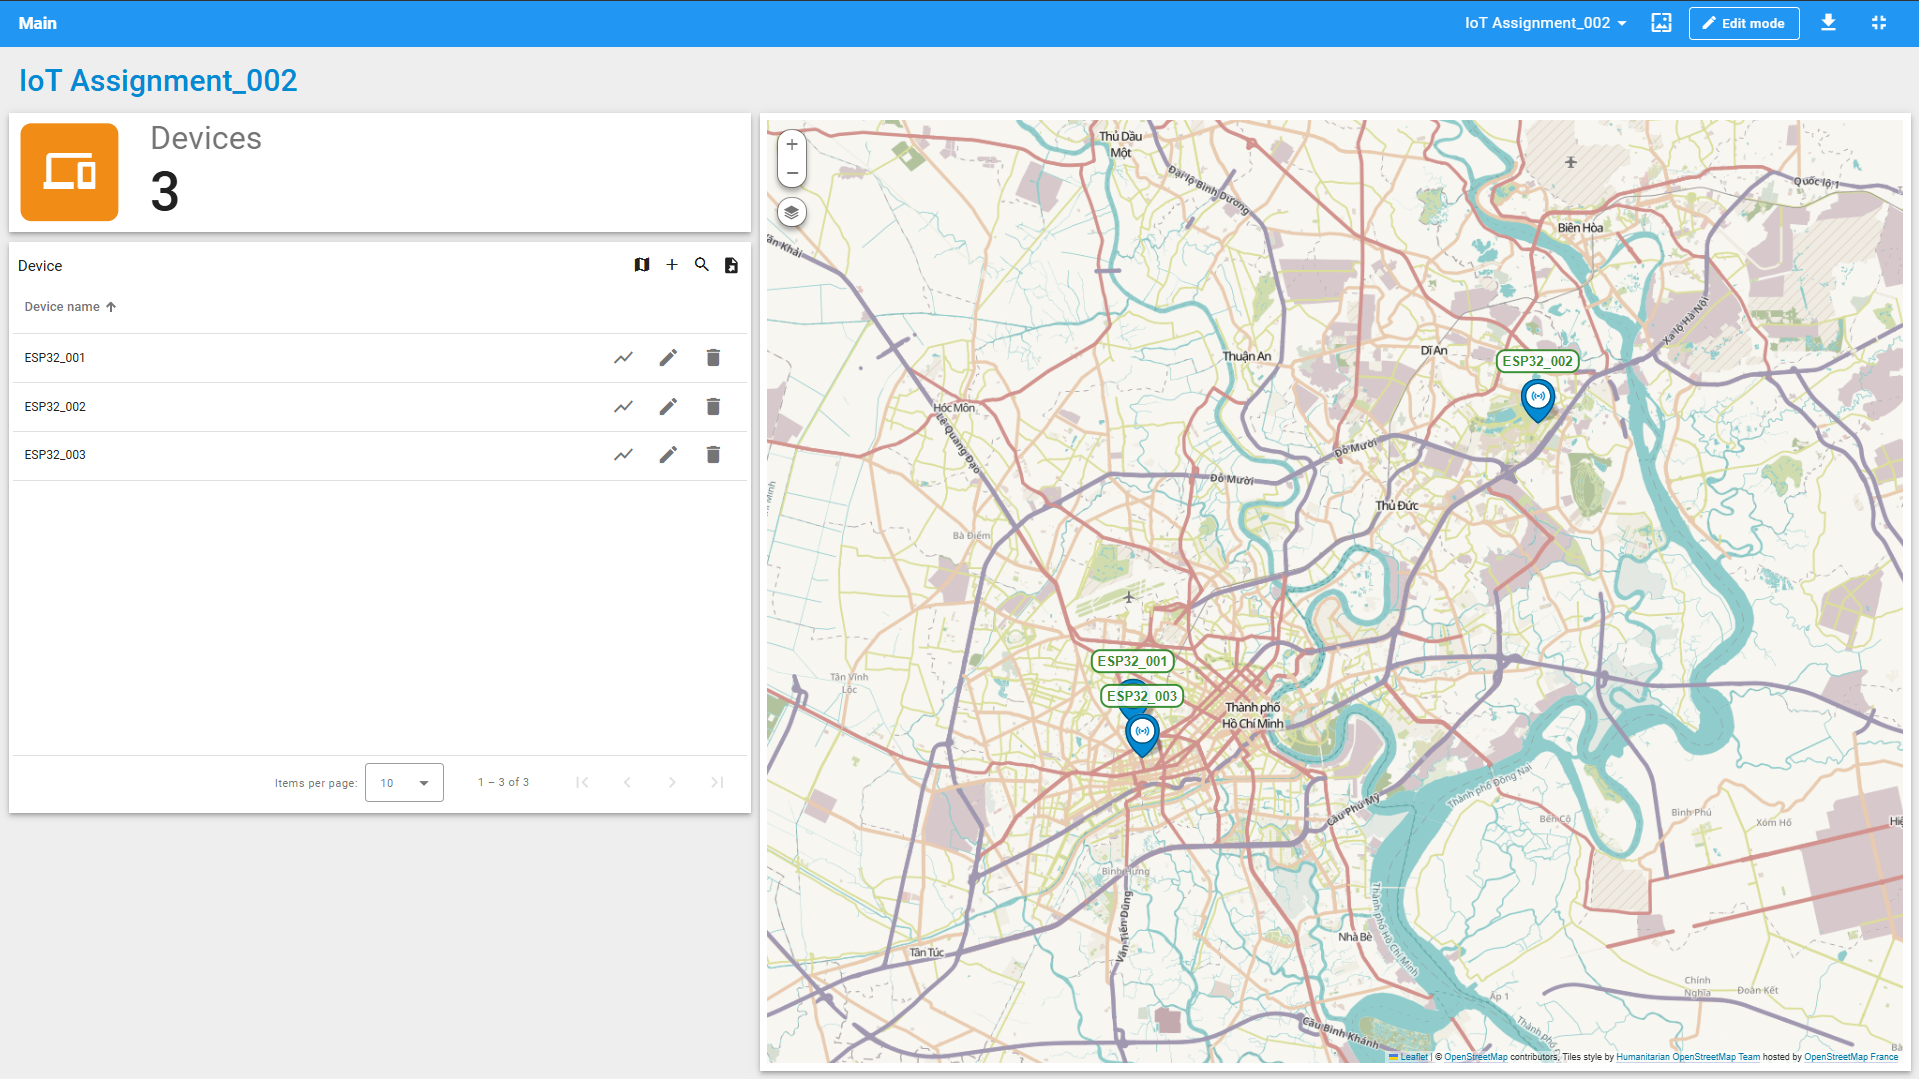
\includegraphics[width=1\textwidth]{pictures/dashboard_001.png}
    \caption{Giao diện mặc định của Dashboard}
\end{figure}


\begin{figure}[H]
    \centering
    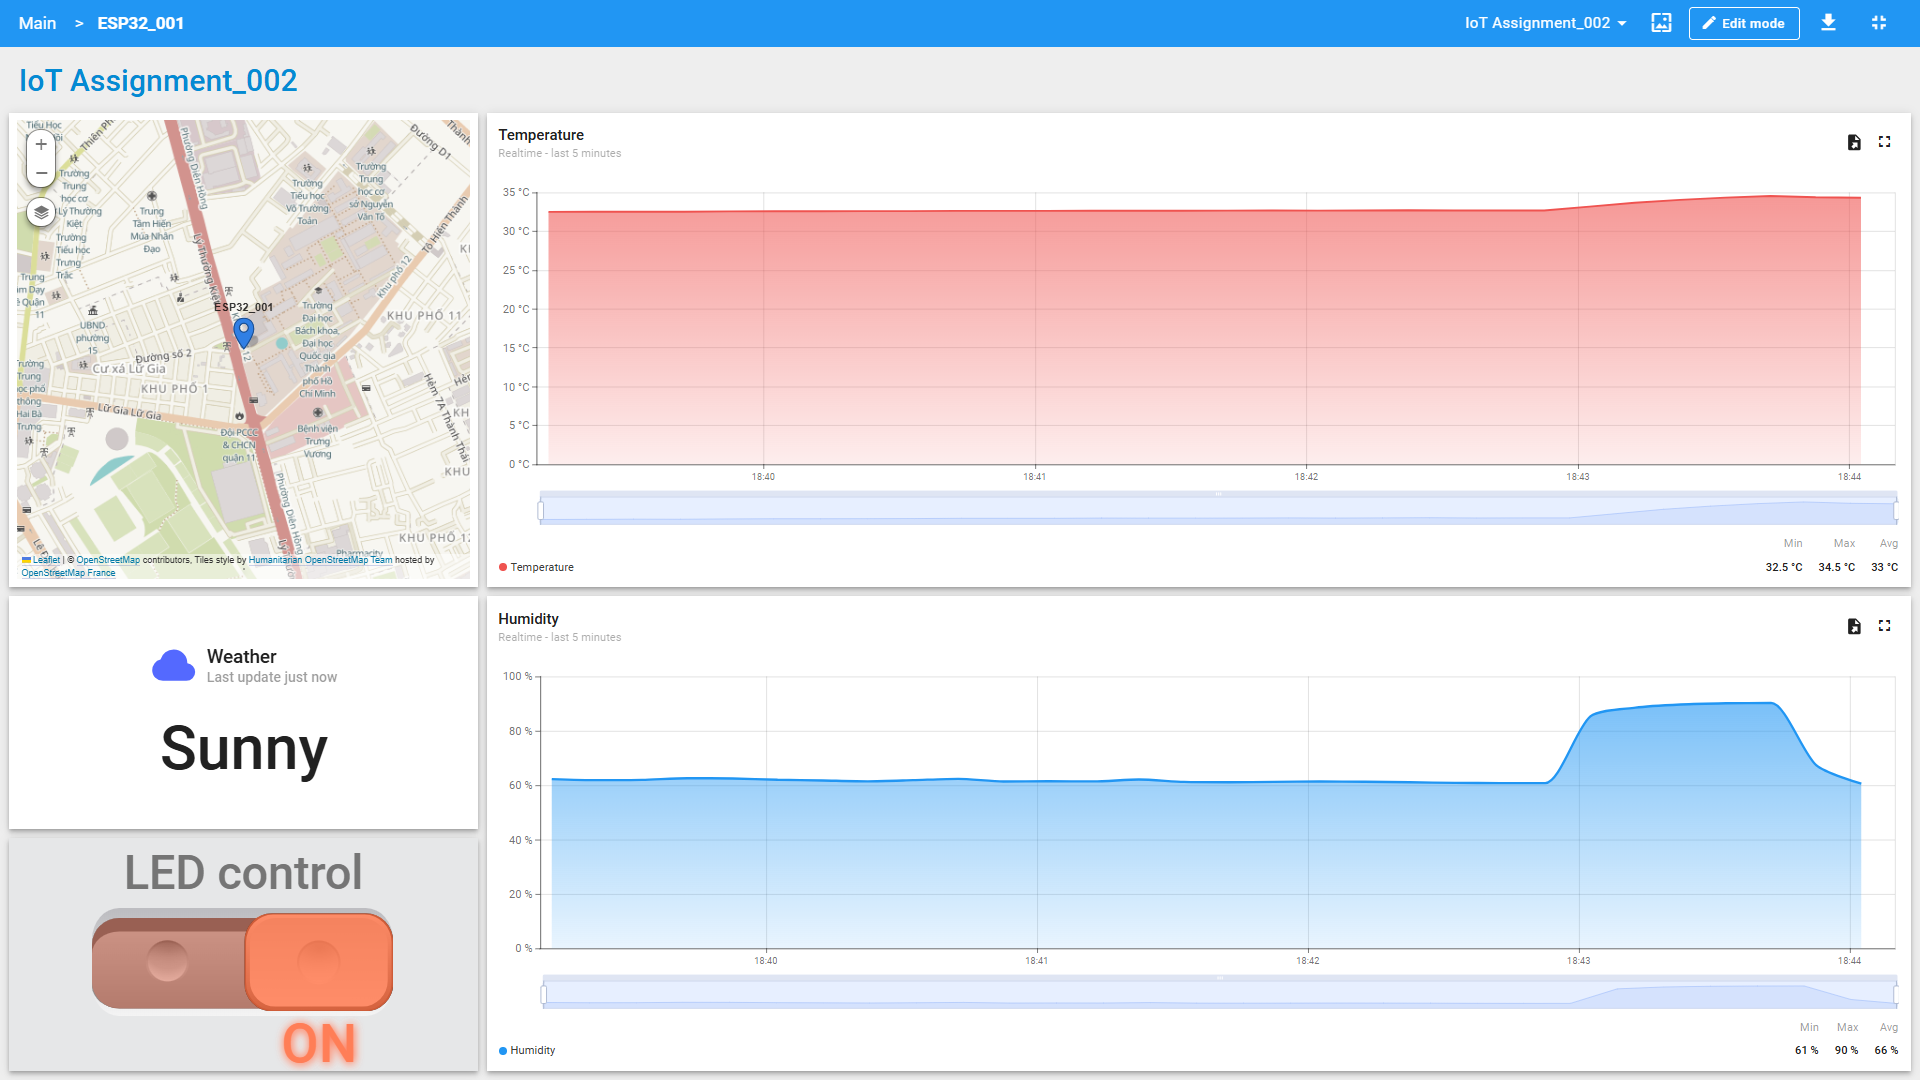
\includegraphics[width=1\textwidth]{pictures/dashboard_002.png}
    \caption{Giao diện Dashboard cho thiết bị ESP32\_001 kết nối với Gateway}
\end{figure}



Dưới đây là các đặc tính kỹ thuật và cấu trúc thành phần của Dashboard "IoT Assignment\_002" với cấu hình chung gồm:

\begin{itemize}
    \item \textit{Giao diện mặc định:} Dashboard được đặt tên là "IoT Assignment\_002" với giao diện mặc định thể hiện các device kết nối với Gateway và vị trí của chúng trên bản đồ, nhằm cho mọi người biết số lượng device cũng như phân bố của chúng.
    \item \textit{Giao diện dữ liệu được gửi từ các device:} Giao diện thứ hai được thể hiện cách thông tin thu thập được từ device như vị trí, nhiệt độ, độ ẩm, kết quả của TinyML. Cùng với đó là sự xuất hiện của một Button gửi tín hiệu RPC về cho ESP32, theo như thiết kế đây là nơi sẽ quyết định LED đơn có bật hay tắt hay không.
\end{itemize}


\subsubsection{Cơ chế gửi email - Rule chain}

Hệ thống điều khiển và giám sát sử dụng công cụ Rule Chain của CoreIOT để thiết lập một quy trình xử lý dữ liệu tự động. Quy trình này không chỉ dừng lại ở việc lưu trữ dữ liệu mà còn thực hiện các phép tính thống kê và gửi báo cáo định kỳ qua Email cho người quản lý. 

\begin{figure}[H]
    \centering
    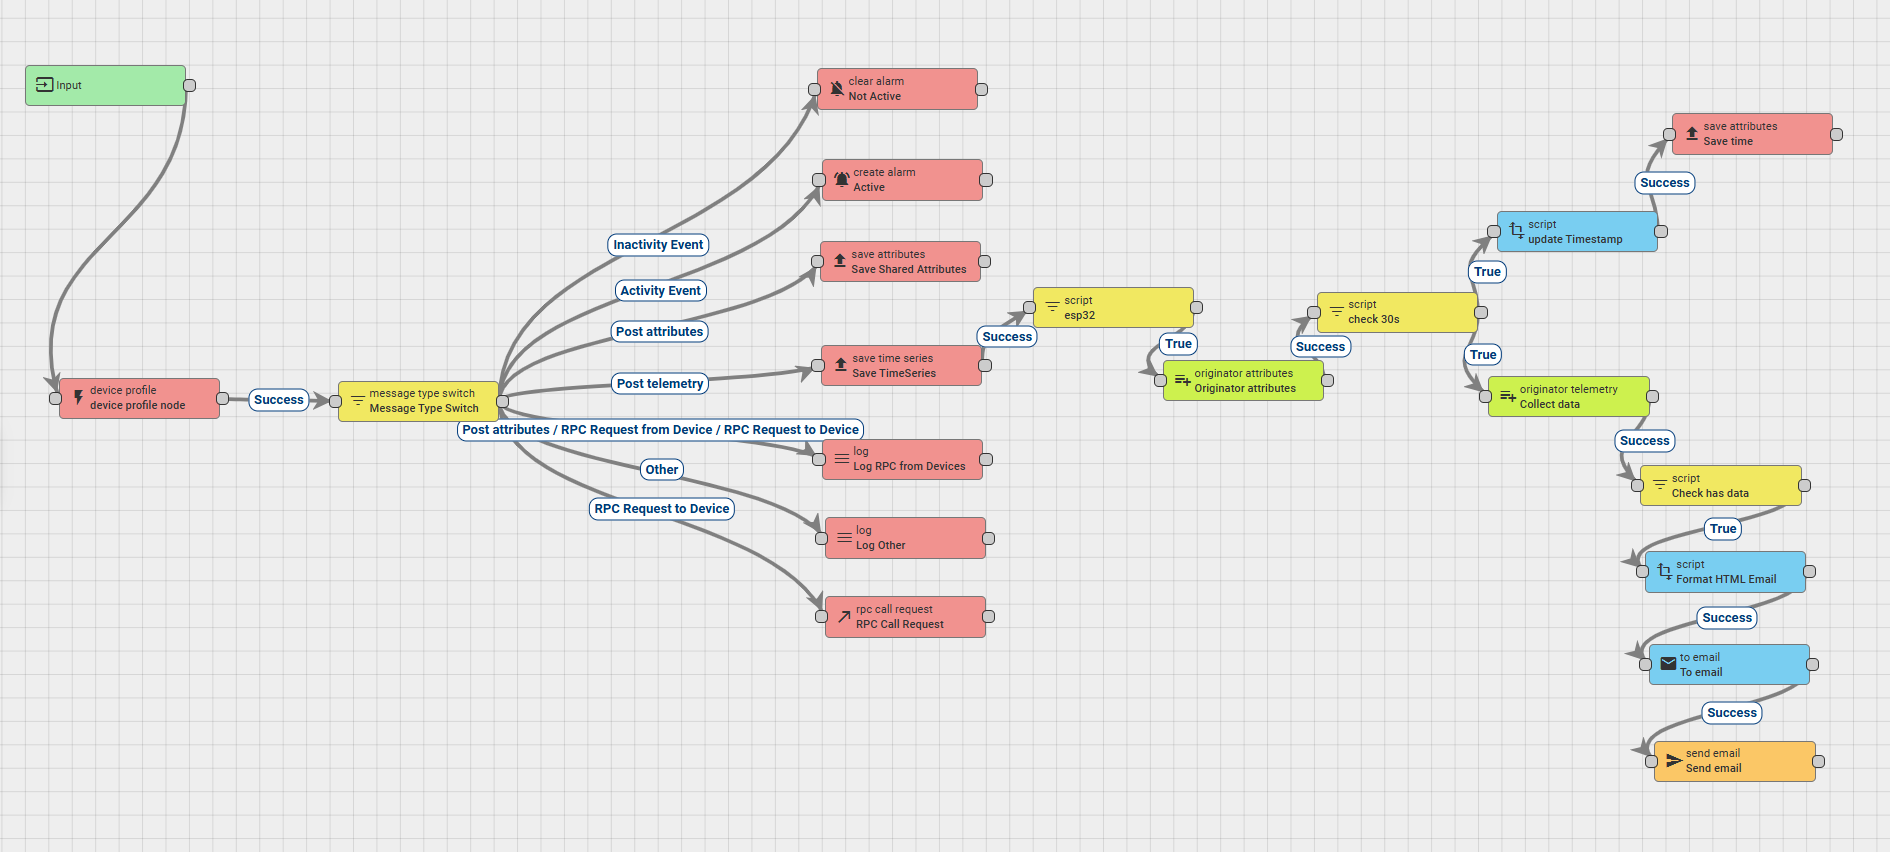
\includegraphics[width=1\textwidth]{pictures/rulechain.png}
    \caption{Rule chain hiện thực cớ chế gửi email}
\end{figure}




Dưới đây là phân tích chi tiết các khối chức năng (Nodes) trong Rule Chain "Gateway":

\begin{itemize}
    \item \textbf{Khối phân loại và lưu trữ cơ sở:}
    \begin{itemize}
        \item \textit{Message Type Switch:} Đây là node điều hướng trung tâm, có nhiệm vụ phân loại các bản tin đến. Các bản tin thuộc loại "Post telemetry" (dữ liệu cảm biến) sẽ được dẫn hướng tới các bước xử lý báo cáo.
        \item \textit{Save TimeSeries:} Thực hiện lưu trữ dữ liệu nhiệt độ, độ ẩm vào cơ sở dữ liệu để hiển thị lên Dashboard. Chỉ khi dữ liệu được lưu thành công, luồng gửi email mới được kích hoạt qua nhánh "Success".
    \end{itemize}

    \item \textbf{Khối lọc thiết bị và kiểm soát tần suất (Rate Limiting):}
    \begin{itemize}
        \item \textit{esp32 (Filter Node):} Sử dụng mã JavaScript để kiểm tra tên thiết bị có phải ESP32 hay không. Điều này đảm bảo hệ thống chỉ xử lý báo cáo cho các node cảm biến ESP32 mà không bị lẫn với các thiết bị khác.
        \item \textit{Originator attributes \& check 30s:} Hai khối này phối hợp để ngăn chặn việc gửi email quá dồn dập. Hệ thống truy xuất thuộc tính \texttt{last\_email\_time} từ server và so sánh với thời gian hiện tại. Theo logic code quy định khoảng cách giữa 2 lần gửi phải $\ge$ 30,000ms.
    \end{itemize}

    \item \textbf{Khối truy vấn và xử lý dữ liệu thống kê:}
    \begin{itemize}
        \item \textit{Collect data:} Khi thỏa mãn điều kiện về thời gian, node này sẽ truy vấn ngược lại cơ sở dữ liệu để lấy toàn bộ các điểm dữ liệu \texttt{temperature} và \texttt{humidity} trong vòng 30 giây gần nhất.
        \item \textit{Check has data:} Kiểm tra mảng dữ liệu trả về. Nếu mảng rỗng (không có dữ liệu trong 30 giây qua), quy trình sẽ dừng lại để tránh gửi email trống.
        \item \textit{Format HTML Email:} Đây là khối xử lý phức tạp nhất bằng JavaScript. Nó thực hiện:
        \begin{itemize}
            \item Chuyển đổi Timestamp sang định dạng giờ Việt Nam (HH:mm:ss).
            \item Tính toán giá trị \textbf{Trung bình (Average)} bằng cách lấy tổng chia cho số lượng mẫu.
            \item Tính toán giá trị \textbf{Trung vị (Median)} bằng cách sắp xếp mảng và lấy giá trị ở giữa.
            \item Xây dựng cấu trúc bảng HTML (\texttt{<table>}) để trình bày dữ liệu chuyên nghiệp.
        \end{itemize}
    \end{itemize}

    \item \textbf{Khối thực thi gửi Email:}
    \begin{itemize}
        \item \textit{To email:} Thiết lập các thông số Header cho email như người gửi, người nhận và tiêu đề thư.
        \item \textit{Send email:} Thực hiện việc gửi thư đi thực tế qua internet.
    \end{itemize}
\end{itemize}

\begin{figure}[H]
    \centering
    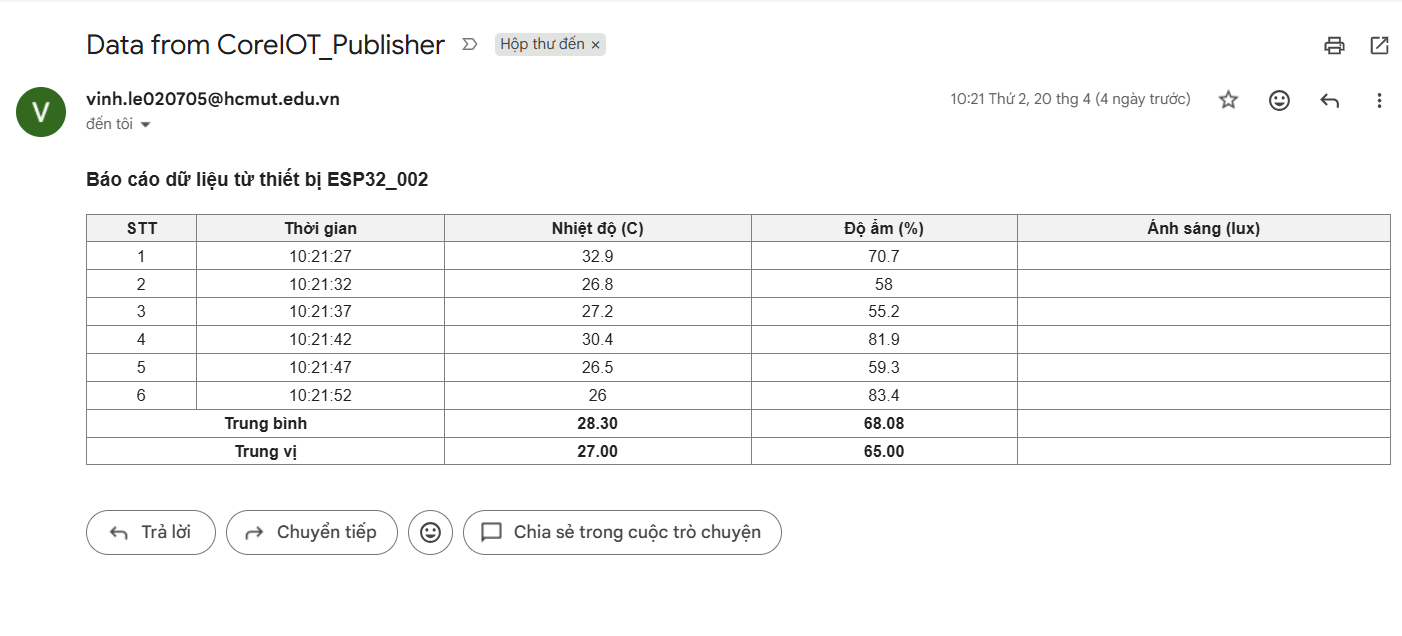
\includegraphics[width=1\textwidth]{pictures/email.png}
    \caption{Email tổng hợp thông tin dữ liệu thu được từ các ESP32}
\end{figure}




\textbf{Đánh giá tổng quan:} Rule Chain này được thiết kế theo mô hình hướng sự kiện (Event-driven). Việc tách biệt luồng cập nhật mốc thời gian và luồng xử lý HTML giúp hệ thống hoạt động ổn định, đảm bảo tính toàn vẹn của dữ liệu báo cáo ngay cả khi lưu lượng dữ liệu từ các node ESP32 gửi về lớn.

\subsection{Cải tiến}


\section{Kết quả thực nghiệm và Đánh giá}
\subsection{Hình ảnh thực tế mô hình}
\subsection{Đánh giá độ chính xác của TinyML}
\subsection{Kết quả kiểm thử}

\section{Kết luận và Hướng phát triển}
\subsection{Kết luận}
Sau quá trình thực hiện dự án, nhóm đã xây dựng thành công một hệ thống IoT hoàn chỉnh trên nền tảng vi điều khiển ESP32 S3. Kết quả đạt được cho thấy sự kết hợp hiệu quả giữa các kỹ thuật lập trình nhúng hiện đại và khả năng kết nối điện toán đám mây. Các thành tựu chính của dự án bao gồm:
\begin{itemize}
    \item \textbf{Quản lý tác vụ thời gian thực:} Hệ thống vận hành ổn định nhờ việc áp dụng cơ chế Semaphore để điều phối các nhiệm vụ từ đọc dữ liệu cảm biến đến điều khiển thiết bị ngoại vi. Cách tiếp cận này giúp tối ưu hóa hiệu suất xử lý và loại bỏ triệt để việc sử dụng biến toàn cục trong toàn bộ chương trình.
    \item \textbf{Linh hoạt trong điều khiển và cấu hình:} Web Server được thiết kế cho phép hệ thống tự động chuyển đổi giữa các chế độ mạng khác nhau. Người dùng có thể dễ dàng thiết lập thông số hoặc điều khiển thiết bị thông qua giao diện trực quan ngay trên trình duyệt web.
    \item \textbf{Trí tuệ nhân tạo tại biên:} Nhóm đã hiện thực hóa việc phân loại trạng thái môi trường ngay trên phần cứng bằng mô hình TinyML. Điều này chứng minh khả năng xử lý thông minh của thiết bị nhúng mà không cần phụ thuộc hoàn toàn vào máy chủ bên ngoài.
    \item \textbf{Tích hợp hệ sinh thái đám mây:} Dữ liệu môi trường được truyền tải liên tục và bảo mật lên máy chủ CoreIOT. Các tính năng mở rộng như cập nhật phần mềm từ xa và thông báo khẩn cấp qua email đã được triển khai đầy đủ theo yêu cầu kỹ thuật.
\end{itemize}
Dự án đã giúp các thành viên nắm vững quy trình phát triển một sản phẩm IoT thực tế, từ khâu thiết kế phần cứng đến lập trình phần mềm đa nhiệm.

\subsection{Hướng phát triển tương lai}
Dựa trên nền tảng sẵn có, hệ thống có thể được tiếp tục cải tiến và mở rộng theo các hướng chủ đạo như sau:
\begin{itemize}
    \item \textbf{Tối ưu hóa thuật toán học máy:} Nhóm dự kiến thu thập tập dữ liệu lớn hơn với nhiều biến số môi trường để huấn luyện các mô hình mạng nơ-ron sâu. Việc này sẽ giúp nâng cao độ chính xác khi dự báo các tình huống bất thường và giảm thiểu sai số trong các môi trường khắc nghiệt.
    \item \textbf{Nâng cao hiệu quả sử dụng năng lượng:} Nghiên cứu và áp dụng các chế độ tiết kiệm điện chuyên sâu là hướng đi quan trọng để kéo dài thời gian hoạt động của thiết bị khi sử dụng nguồn pin. Hệ thống sẽ được lập trình để chỉ kích hoạt các module truyền thông khi có sự thay đổi đáng kể về dữ liệu.
    \item \textbf{Mở rộng khả năng ứng dụng thực tế:} Hệ thống có thể tích hợp thêm các loại cảm biến đo nồng độ bụi mịn hoặc độ pH của đất để phục vụ cho các giải pháp giám sát môi trường đô thị và nông nghiệp công nghệ cao.
    \item \textbf{Tăng cường bảo mật hệ thống:} Việc áp dụng các giao thức mã hóa dữ liệu đầu cuối và cơ chế xác thực đa lớp sẽ là ưu tiên hàng đầu. Điều này đảm bảo an toàn thông tin khi hệ thống được triển khai trong các mạng lưới quy mô lớn hoặc các khu vực nhạy cảm về dữ liệu.
\end{itemize}

\section*{Tài liệu tham khảo và Phụ lục}


\end{document}